\section{1174079 -Chandra Kirana Poetra}
Chapter 3 - Prediksi dengan Random Forest
\subsection{Teori}
\subsubsection{ Jelaskan apa itu random forest, sertakan gambar ilustrasi buatan sendiri.}
\hfill\\
Random forest merupakan algorithma klasifikasi yang meliputi banyak decisions tress. random forest menggunakan bangging (salah satu algoritma machine learning) serta fitur pengacakan(randomness) ketika membangun setiap satu tree untuk mencoba membuat suatu hutan yang berisi pohon yang tidak berkorelasi

\begin{figure}[H]
	\centering
	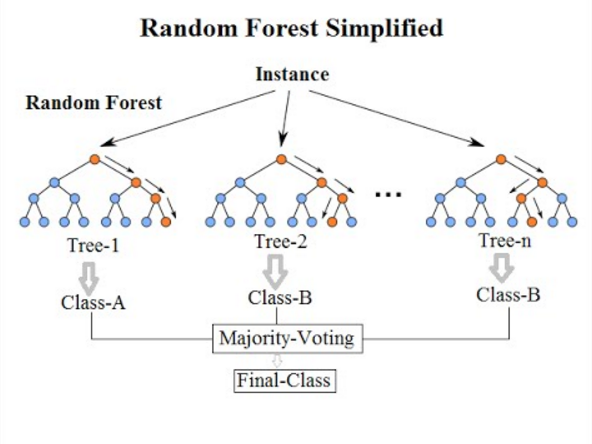
\includegraphics[width=12cm]{figures/1174079/3/randomforest.png}
	\caption{contoh random forest}
\end{figure}


\subsubsection{Jelaskan cara membaca dataset kasus dan artikan makna setiap file dan isi field masing masing file.}
\hfill\\
Dataset adalah suatu koleksi dari banyak data, biasanya dalam bentuk tabel dan penggambarannya kurang lebih mirip seperti table yang ada di database.
\begin{enumerate}
\item cara membaca dataset
\hfill\\
\lstinputlisting[]{src/1174079/3/bacadataset.py}
	\begin{itemize}
	\item import library panda dan namai sebagai pd agar memudahkan pemanggilan
	\item buat variable dataset dan panggil perintah untuk membaca file yang dimaksud
	\hfill\\	
	\item berikut hasilnya
	\hfill\\
\begin{figure}[H]
	\centering
	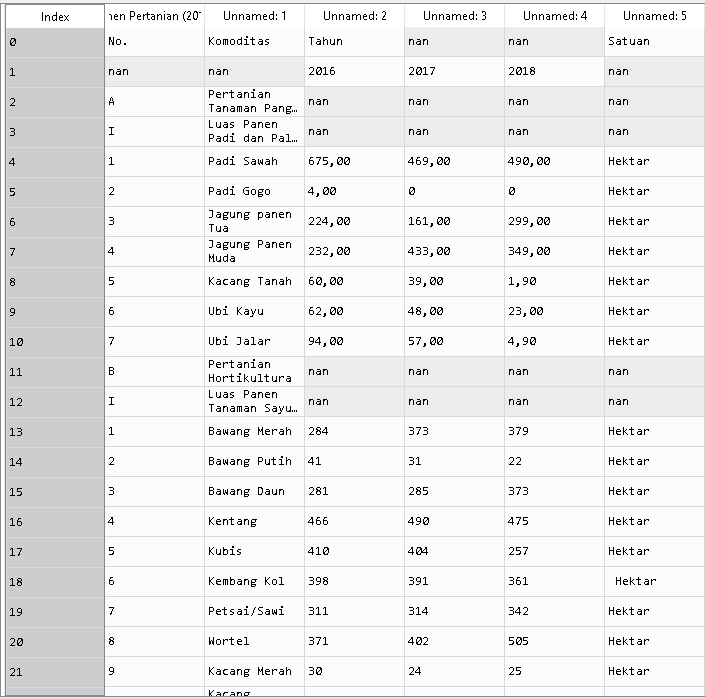
\includegraphics[width=12cm]{figures/1174079/3/hasilbacadataset.PNG}
	\caption{contoh dataset}
\end{figure}
\end{itemize}
\end{enumerate}

\subsubsection{ Jelaskan apa itu cross validation}
\hfill\\
Cross-validation (CV) adalah Merupakan metode statistic untuk meng-evaluasi dan membandingkan akurasi Learning algorithm dengan cara membagi dataset menjadi 2 bagian: Satu bagian digunakan untuk training model, Bagian yang lain untuk mem-validasi model Suatu dataset akan dibagi sesuai dengan banyaknya k, dan akan di test bergantian hingga seluruh bagian terpenuhi.

\subsubsection{Jelaskan apa arti score 44\% pada random forest, 27\% pada decission tree dan 29\% dari SVM.}
\hfill\\
Score dari masing masing itu merupakan hasil dari tingkat keakuratan predikasi yang digunakan, jika menggunakan random forest anda mendapatkan tingkat keakuratan mencapai 44\%, decision tree sekitar 27\% dan svm 29\%.

\subsubsection{Jelaskan bagaimana cara membaca confusion matriks dan contohnya memakai gambar atau ilustrasi sendiri.}
\begin{figure}[H]
	\centering
	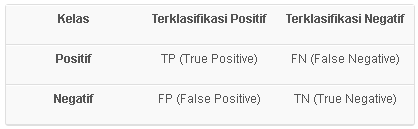
\includegraphics{figures/1174079/3/carabacaconfusionmatrix.PNG}
	\caption{Contoh confusion matrix}
\end{figure}
\begin{enumerate}
\item TP adalah True Positive, jumlah data positif terdeteksi benar 
\item TN adalah True Negative,  jumlah data negatif terdeteksi benar.
\item FN adalah False Negative,  jumlah data negatif terdeteksi salah.
\item FP adalah False Positive,  jumlah data positif terdeteksi salah 
\end{enumerate}
\begin{figure}[H]
	\centering
	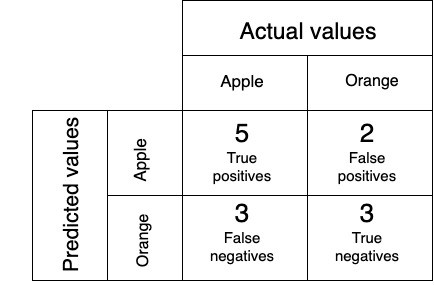
\includegraphics{figures/1174079/3/contohconfusionmatrix.jpeg}
	\caption{Contoh confusion matrix}
\end{figure}
Penjelasan dari gambar diatas adalah mesin mendeteksi 5 apel sebagai 5 apel dan 2 apel sisanya terdeteksi sebagai jeruk, lalu 3 jeruk terdeteksi sebagai apel dan 3 jeruk terdeteksi sebagai jeruk.


\subsubsection{Jelaskan apa itu voting pada random forest disertai dengan ilustrasi gambar sendiri.}
\hfill\\
Voting di random forest kurang lebih sama seperti ketika kita ingin bertanya atau survey apakah suatu makanan masuk ke kategori enak atau tidak, jadi bisa dibilang voting itu adalah suara atau pendapat, yang akan diklasifikasikan.
\begin{figure}[H]
	\centering
	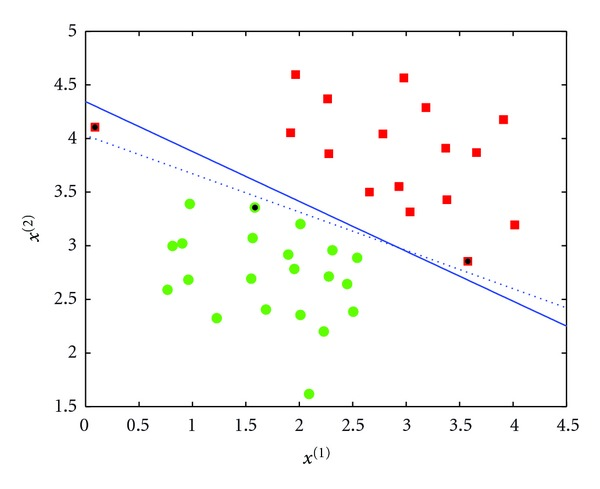
\includegraphics[width=8cm]{figures/1174079/3/klasifikasirandomforest.png}
	\caption{contoh random forest tentang kualitas barang yang semakin mahal semakin tahan lama}
\end{figure}

\subsection{Praktek}

\subsubsection{Nomor 1}
\hfill\break
\lstinputlisting[firstline=8, lastline=12]{src/1174079/3/1174079.py}
\begin{figure}[H]
\centerline{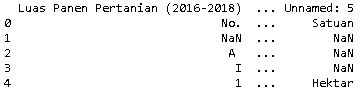
\includegraphics[width=5cm]{figures/1174079/3/praktek0.PNG}}
\caption{Membuat Aplikasi pakai pandas}
\label{labelgambar}
\end{figure}

\subsubsection{Nomor 2}
\hfill\break
\lstinputlisting[firstline=14, lastline=15]{src/1174079/3/1174079.py}
\begin{figure}[H]
\centerline{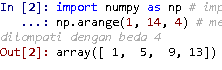
\includegraphics[width=5cm]{figures/1174079/3/praktek1.PNG}}
\caption{Membuat Aplikasi pakai numpy}
\label{labelgambar}
\end{figure}

\subsubsection{Nomor 3}
\hfill\break
\lstinputlisting[firstline=18, lastline=24]{src/1174079/3/1174079.py}
\begin{figure}[H]
\centerline{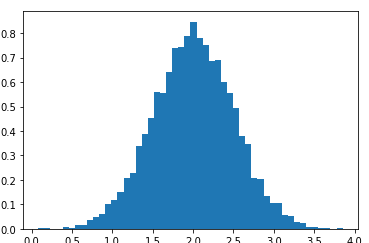
\includegraphics[width=6cm]{figures/1174079/3/praktek2.PNG}}
\caption{Membuat Aplikasi pakai matplotlib}
\label{labelgambar}
\end{figure}

\subsubsection{Nomor 4}
\hfill\break

\begin{itemize}
\item Membaca dataset dengan variable budi. variable ini digunakan untuk mengisi data
\lstinputlisting[firstline=34, lastline=38]{src/1174079/3/1174079.py}
\begin{figure}[H]
\centerline{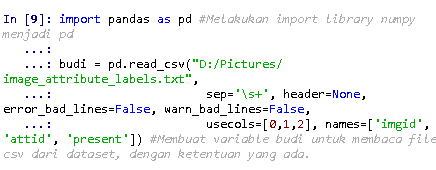
\includegraphics[width=10cm]{figures/1174079/3/praktek3.PNG}}
\caption{Hasil 4 Bagian 1}
\label{labelgambar}
\end{figure}

\item Menampilkan data teratas dari variable budi
\lstinputlisting[firstline=42, lastline=43]{src/1174079/3/1174079.py}
\begin{figure}[H]
\centerline{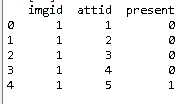
\includegraphics[width=6cm]{figures/1174079/3/praktek4.PNG}}
\caption{Hasil 4 Bagian 2}
\label{labelgambar}
\end{figure}

\item menampilkan jumlah kolum dan baris dari varaible budi
\lstinputlisting[firstline=45, lastline=45]{src/1174079/3/1174079.py}
\begin{figure}[H]
\centerline{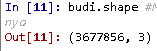
\includegraphics[width=5cm]{figures/1174079/3/praktek5.PNG}}
\caption{Hasil 4 Bagian 3}
\label{labelgambar}
\end{figure}

\item Mengubah kolum jadi baris dengan fungsi pivot yang disimpan pada variable budi2 yang datanya berasal dari variable budi sebelumnya.
\lstinputlisting[firstline=48, lastline=48]{src/1174079/3/1174079.py}
\begin{figure}[H]
\centerline{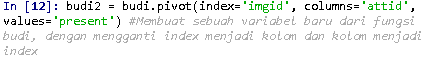
\includegraphics[width=5cm]{figures/1174079/3/praktek6.PNG}}
\caption{Hasil 4 Bagian 4}
\label{labelgambar}
\end{figure}

\item Menampilkan data teratas dari budi2
\lstinputlisting[firstline=51, lastline=51]{src/1174079/3/1174079.py}
\begin{figure}[H]
\centerline{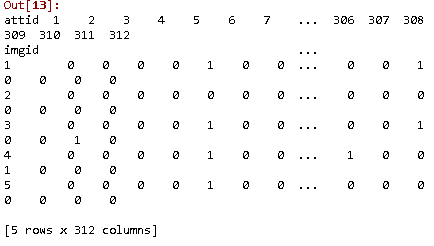
\includegraphics[width=5cm]{figures/1174079/3/praktek7.PNG}}
\caption{Hasil 4 Bagian 5}
\label{labelgambar}
\end{figure}

\item menampilkan jumlah kolumm dan baris variable budi2
\lstinputlisting[firstline=54, lastline=54]{src/1174079/3/1174079.py}
\begin{figure}[H]
\centerline{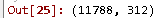
\includegraphics[width=5cm]{figures/1174079/3/praktek8.PNG}}
\caption{Hasil 4 Bagian 6}
\label{labelgambar}
\end{figure}

\item membaca data csv dan membuat index baru bernama imgid
\lstinputlisting[firstline=56, lastline=59]{src/1174079/3/1174079.py}
\begin{figure}[H]
\centerline{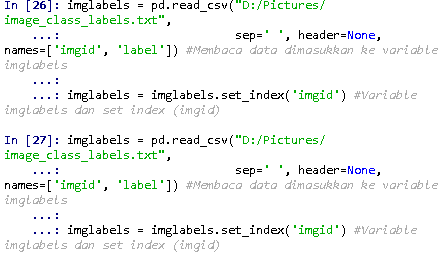
\includegraphics[width=5cm]{figures/1174079/3/praktek9.PNG}}
\caption{Hasil 4 Bagian 7}
\label{labelgambar}
\end{figure}

\item Menampilkan data teratas
\lstinputlisting[firstline=62, lastline=62]{src/1174079/3/1174079.py}
\begin{figure}[H]
\centerline{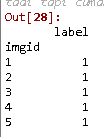
\includegraphics[width=5cm]{figures/1174079/3/praktek10.PNG}}
\caption{Hasil 4 Bagian 8}
\label{labelgambar}
\end{figure}

\item mengeluarkan output jumlah kolumm dan baris
\lstinputlisting[firstline=65, lastline=65]{src/1174079/3/1174079.py}
\begin{figure}[H]
\centerline{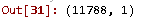
\includegraphics[width=5cm]{figures/1174079/3/praktek11.PNG}}
\caption{Hasil 4 Bagian 9}
\label{labelgambar}
\end{figure}

\item Menggabungkan variable budi2 dan imglabels karena isi yang mirip sehingga bisa dikategorikan sebagai supervised learning.
\lstinputlisting[firstline=68, lastline=69]{src/1174079/3/1174079.py}
\begin{figure}[H]
\centerline{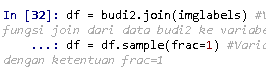
\includegraphics[width=5cm]{figures/1174079/3/praktek12.PNG}}
\caption{Hasil 4 Bagian 10}
\label{labelgambar}
\end{figure}

\item membuat columm
\lstinputlisting[firstline=72, lastline=73]{src/1174079/3/1174079.py}
\begin{figure}[H]
\centerline{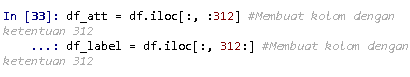
\includegraphics[width=5cm]{figures/1174079/3/praktek13.PNG}}
\caption{Hasil 4 Bagian 11}
\label{labelgambar}
\end{figure}

\item Mengecek data teratas variable df\_att.
\lstinputlisting[firstline=76, lastline=76]{src/1174079/3/1174079.py}
\begin{figure}[H]
\centerline{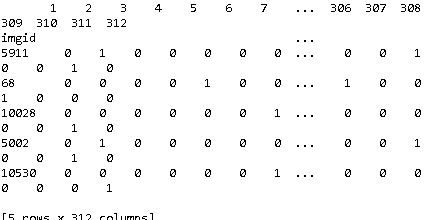
\includegraphics[width=5cm]{figures/1174079/3/praktek14.PNG}}
\caption{Hasil 4 Bagian 12}
\label{labelgambar}
\end{figure}

\item Mengeceki data teratas dari df\_label.
\lstinputlisting[firstline=79, lastline=79]{src/1174079/3/1174079.py}
\begin{figure}[H]
\centerline{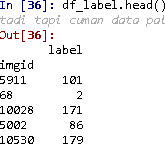
\includegraphics[width=5cm]{figures/1174079/3/praktek15.PNG}}
\caption{Hasil 4 Bagian 13}
\label{labelgambar}
\end{figure}

\item Membagi 8000 baris awal sebagai data training dan yang lainnya sebagai data testing.
\lstinputlisting[firstline=82, lastline=88]{src/1174079/3/1174079.py}
\begin{figure}[H]
\centerline{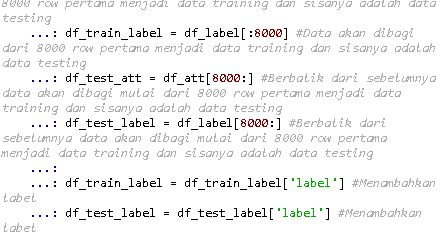
\includegraphics[width=5cm]{figures/1174079/3/praktek16.PNG}}
\caption{Hasil 4 Bagian 14}
\label{labelgambar}
\end{figure}

\item memanggil class RandomForestClassifier. dengan maks kolum 50
\lstinputlisting[firstline=91, lastline=92]{src/1174079/3/1174079.py}
\begin{figure}[H]
\centerline{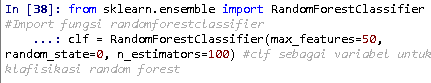
\includegraphics[width=5cm]{figures/1174079/3/praktek17.PNG}}
\caption{Hasil 4 Bagian 15}
\label{labelgambar}
\end{figure}

\item output hasil prediksi dari Random Forest.
\lstinputlisting[firstline=95, lastline=95]{src/1174079/3/1174079.py}
\begin{figure}[H]
\centerline{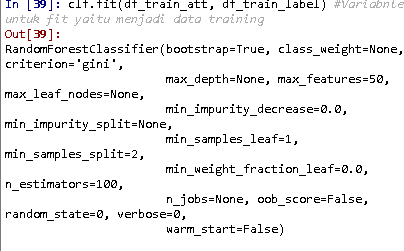
\includegraphics[width=5cm]{figures/1174079/3/praktek18.PNG}}
\caption{Hasil 4 Bagian 16}
\label{labelgambar}
\end{figure}

\item Memperlihatkan score akurasi.
\lstinputlisting[firstline=98, lastline=98]{src/1174079/3/1174079.py}
\begin{figure}[H]
\centerline{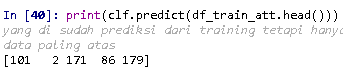
\includegraphics[width=5cm]{figures/1174079/3/praktek19.PNG}}
\caption{Hasil 4 Bagian 17}
\label{labelgambar}
\end{figure}

\item Menampilkan tingkat akurasi
\lstinputlisting[firstline=101, lastline=101]{src/1174079/3/1174079.py}
\begin{figure}[H]
\centerline{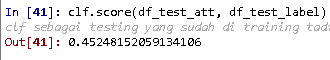
\includegraphics[width=5cm]{figures/1174079/3/praktek20.PNG}}
\caption{Hasil 4 Bagian 18}
\label{labelgambar}
\end{figure}
\end{itemize}

\subsubsection{Nomor 5}
\hfill\break
\lstinputlisting[firstline=112, lastline=114]{src/1174079/3/1174079.py}
\begin{figure}[H]
\centerline{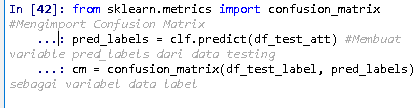
\includegraphics[width=5cm]{figures/1174079/3/praktek21.PNG}}
\caption{Hasil 5 Bagian 1}
\label{labelgambar}
\end{figure}

\lstinputlisting[firstline=117, lastline=117]{src/1174079/3/1174079.py}
\begin{figure}[H]
\centerline{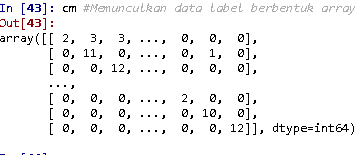
\includegraphics[width=5cm]{figures/1174079/3/praktek22.PNG}}
\caption{Hasil 5 Bagian 2}
\label{labelgambar}
\end{figure}

\lstinputlisting[firstline=120, lastline=147]{src/1174079/3/1174079.py}
\begin{figure}[H]
\centerline{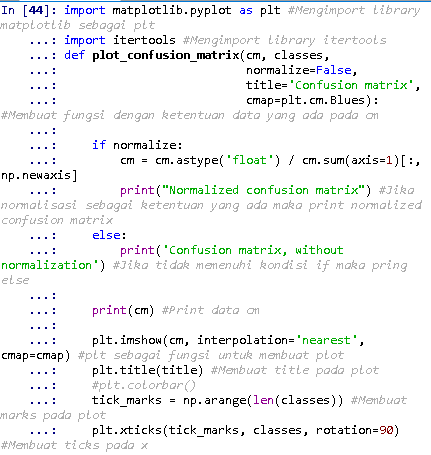
\includegraphics[width=5cm]{figures/1174079/3/praktek23.PNG}}
\caption{Hasil 5 Bagian 3}
\label{labelgambar}
\end{figure}

\lstinputlisting[firstline=151, lastline=154]{src/1174079/3/1174079.py}
\begin{figure}[H]
\centerline{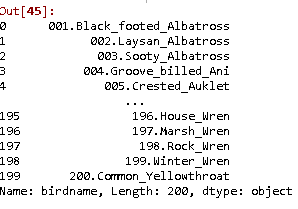
\includegraphics[width=5cm]{figures/1174079/3/praktek24.PNG}}
\caption{Hasil 5 Bagian 4}
\label{labelgambar}
\end{figure}

\lstinputlisting[firstline=158, lastline=163]{src/1174079/3/1174079.py}
\begin{figure}[H]
\centerline{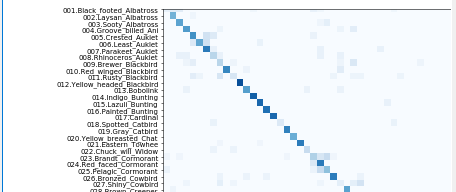
\includegraphics[width=5cm]{figures/1174079/3/praktek25.PNG}}
\caption{Hasil 5 Bagian 5}
\label{labelgambar}
\end{figure}

\subsubsection{Nomor 6}
\hfill\break
\lstinputlisting[firstline=168, lastline=171]{src/1174079/3/1174079.py}
\begin{figure}[H]
\centerline{
\includegraphics[width=5cm]{figures/1174079/3/praktek26.PNG}}
\caption{Hasil 6 Bagian 1}
\label{labelgambar}
\end{figure}

\lstinputlisting[firstline=174, lastline=177]{src/1174079/3/1174079.py}
\begin{figure}[H]
\centerline{
\includegraphics[width=5cm]{figures/1174079/3/praktek27.PNG}}
\caption{Hasil 6 Bagian 2}
\label{labelgambar}
\end{figure}

\subsubsection{Nomor 7}
\hfill\break
\lstinputlisting[firstline=180, lastline=182]{src/1174079/3/1174079.py}
\begin{figure}[H]
\centerline{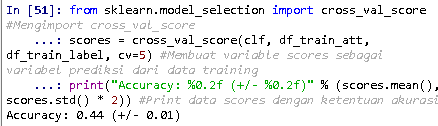
\includegraphics[width=5cm]{figures/1174079/3/praktek28.PNG}}
\caption{Hasil 7 Bagian 1}
\label{labelgambar}
\end{figure}

\lstinputlisting[firstline=185, lastline=186]{src/1174079/3/1174079.py}
\begin{figure}[H]
\centerline{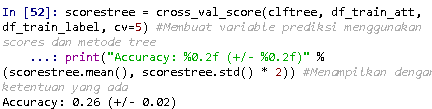
\includegraphics[width=5cm]{figures/1174079/3/praktek29.PNG}}
\caption{Hasil 7 Bagian 2}
\label{labelgambar}
\end{figure}

\lstinputlisting[firstline=189, lastline=190]{src/1174079/3/1174079.py}
\begin{figure}[H]
\centerline{
\includegraphics[width=5cm]{figures/1174079/3/praktek30.PNG}}
\caption{Hasil 7 Bagian 3}
\label{labelgambar}
\end{figure}

\subsubsection{Nomor 8}
\hfill\break
\lstinputlisting[firstline=193, lastline=208]{src/1174079/3/1174079.py}
\begin{figure}[H]
\centerline{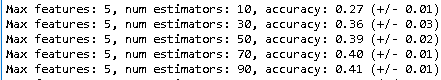
\includegraphics[width=5cm]{figures/1174079/3/praktek31.PNG}}
\caption{Hasil 8 Bagian 1}
\label{labelgambar}
\end{figure}

\lstinputlisting[firstline=210, lastline=224]{src/1174079/3/1174079.py}
\begin{figure}[H]
\centerline{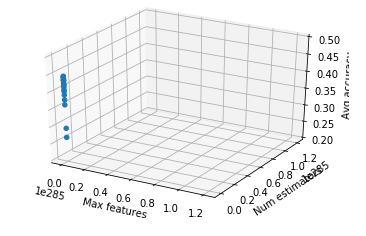
\includegraphics[width=10cm]{figures/1174079/3/praktek32.PNG}}
\caption{Hasil 8 Bagian 2}
\label{labelgambar}
\end{figure}


\subsection{Penanganan Error}
NameError: name 'dataseta' is not defined : Biasanya karena typo, cek lagi penulisan kode

\subsubsection{Tuliskan Kode Error dan Jenis Error}
NameError: name 'dataseta' is not defined

\subsubsection{Cara Penanganan Error}
Pastikan untuk tidak menulis function secara typo dan ceklagi

\subsubsection{Bukti Tidak Plagiat}
\hfill\\
\begin{figure}[H]
	\centering
	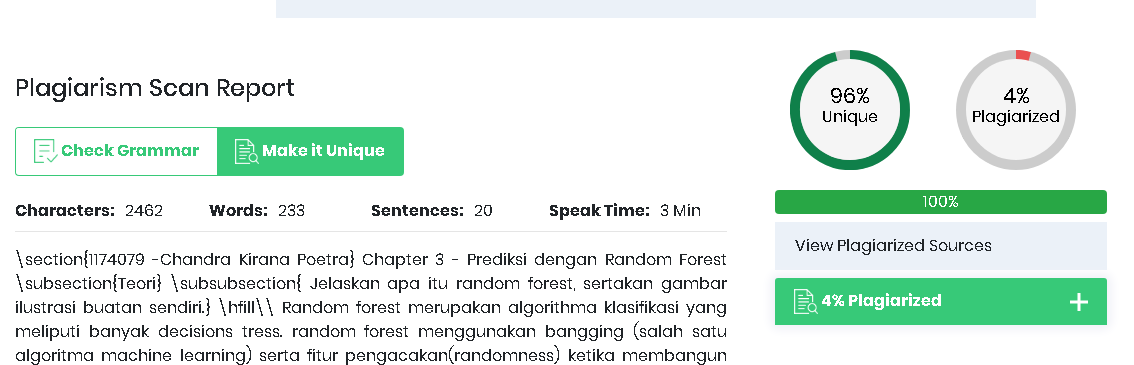
\includegraphics[width=12cm]{figures/1174079/3/plagiarismchecker.PNG}
	\caption{Cek Plagiarism}
\end{figure}


\subsection{Link Video Youtube}
https://youtu.be/hWCR0dXYagk